\documentclass[UTF8]{ctexart}
\usepackage[T1]{fontenc}

% Language setting
% Replace `english' with e.g. `spanish' to change the document language
\usepackage[english]{babel}
\usepackage{color}

% Set page size and margins
% Replace `letterpaper' with `a4paper' for UK/EU standard size
\usepackage[letterpaper,top=2cm,bottom=2cm,left=3cm,right=3cm,marginparwidth=1.75cm]{geometry}

% Useful packages
\usepackage{amsmath}
\usepackage{graphicx}
\usepackage{array}
\usepackage{longtable}

\usepackage[colorlinks=true, allcolors=blue]{hyperref}

\title{多立恒网页使用指南}
\author{司迎}
% \date{2024年12月6日}
\begin{document}
\maketitle
\tableofcontents
\begin{abstract}
这个文档包含多立恒3.0网页使用时的各种功能说明,以及需要注意的事项。使用时可点击对应索引查看,或使用ctrl+F直接在页面内关键字搜索。
\end{abstract}

\section{首页}

首页左上角展示默认仪表盘,展示内容根据角色权限可以自行调整,管理员默认可以查看所有信息,但也可以在角色权限内调整。

除了角色权限内所显示的版块外,默认仪表盘处点开也可“新建仪表盘”,自定义使用页面首页需要展示的内容,并且可随时展示各种版本页面。首页仪表盘编辑见Figure \ref{fig:preface1}

首页右上角的“通知公告”可以点开查看网页有哪些最近的更新,有些功能需求的上线通知会列在里面。
\begin{figure}[h]
	\centering
	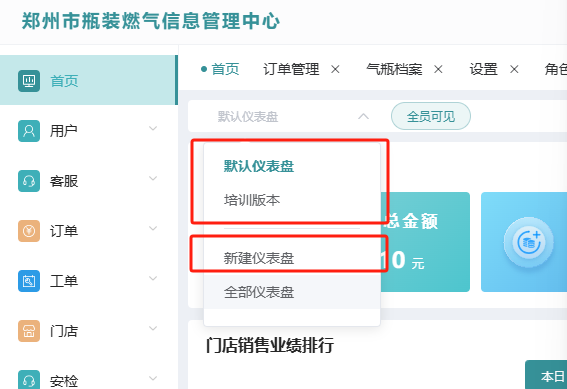
\includegraphics[width=0.7\linewidth]{D:/latex/dlh_tutorial_figs/preface1}
	\caption{首页仪表盘}
	\label{fig:preface1}
\end{figure}

多立恒网页所有可查询的页面都能自定义设置显示列,也可以设置查询框中的默认查询条件。

注意:有些页面的时间类查询条件,系统有默认当天的值,并且不展开查询框就无法直接看到那个查询条件。因此,如果你未设置过查询条件,可能会在不知情的情况下找不到你要查询的内容。出现这类情况可先展开所有的查询条件,排查是否有已写入的值,删掉查询条件内容或者选择你所需的查询条件,再次点击查询即可显示有效信息。

\section{用户}

\subsection{用户管理}
从用户管理中可以查看所有已开户的用户信息,可根据上方的查询条件查询,并导出正式用户表格。用户管理无法通过户号查询。每个用户信息条目右侧可以进行编辑等操作。

用户户号等蓝色标识的内容均可点击进入详细页面,其中比较常用的是“户号”中的内容,可在其中查看用户信息,全部的押金信息,合同信息,订单信息,在用气瓶,以及安检记录等。

\subsection{保单管理}
公司无保险业务,未使用此功能。

\subsection{押金管理}
新郑公司财务不使用此功能,一般信息部作为核查使用。这个功能不好用的点在于拍照内容需要人工审核,押金单内容与拍照的纸质押金单内容不一定一致,有参考价值,但如果作为实际押金收据的证明则因存在监管漏洞而不适用。

包含“正常单据”,“已作废”两个页面,可填充查询条件筛选押金数据。

押金管理可新增押金单,携瓶入户,批量作废,批量回执,导出。列表中,蓝色字体的押金单号和户号可以点开查看详细信息。

每条押金单信息可新增,编辑,作废,退瓶,回执,打印。押金单的编辑功能可编辑所属机构、气瓶类型、数量、押金单价、租金、起租日期、支付方式、经办人、修改或删除、新增押金单照片。用户信息和随单生成的押金单号不能修改。

退瓶功能关联配送员好运气app中的退瓶功能,确认退瓶后会生成一个退瓶单号,对应配送员的手机app中会接到退瓶单并且上门扫码退瓶。押金退款只能走现金途径,无法直接从微信中退回。已退气瓶的退瓶单会更新在“退瓶管理”模块中。

\subsection{退瓶管理}

退瓶后的信息在退瓶管理中更新,可通过退瓶单号、押金单号等相关项查询,退瓶需在网页端手动点确认。

\subsection{欠瓶管理}

一般情况下不允许欠瓶,在随单的“新增欠瓶”功能可自主配置之前,会有配送员在实际操作中本应“新增押金”而错选成了欠瓶,这类情况需要库房营业员将这些欠瓶单全部作废,并按相应的用户和商品规格数量新增押金单,保证数据正常。

\subsection{合同管理}

每个用户都需要跟公司签署供气协议,供气协议上传在合同模板,配置在随单任务中。未签署合同的用户在他的新订单完成前,会与随单安检一起列在随单任务中;已签署合同的用户则不需要再签,签合同入口也不会在随单任务中出现。点开合同编号可查看合同详情。

\textcolor{red}{注意}:
合同管理需要经常(一般是每天)筛选“待我方签署”的合同,批量选择完成签署,用户的合同才会被盖上电子公章。同时,有些早期积压的“待客户签署”的合同,也需要定期找到并撤销,以免后续配送员为这个用户新签合同时导致“用户已发起过相同模板”的提示。



\section{客服}

\subsection{通话分析}


\subsection{通话记录}


\section{订单}

订单是与配送工作关联最大的模块。客服、营业员、运维人员最主要关注的就是这个模块。
\begin{itemize}
	\item \textbf{订单管理}一个订单生成后,会分别进入待指派--配送中--待签单--已签收的流程,若订单生成后未完成,微信未支付取消,或代客下单取消的订单,会生成在“已关闭”选项卡中。
将订单的各个流程状态分别展示在不同的选项卡中以供查询;
    \item \textbf{订单售后}是已支付的订单,在订单完成前从用户端申请退单的订单信息。
\end{itemize}
\subsection{订单管理}

订单管理的字段包含几乎所有订单、用户、气瓶流转信息。只是检索框处并没有将所有字段设置进去以供查询,尤其是无法使用用户户号查询这一项,还是造成了一定程度的不便。

Tips: 有订单管理权限即可看到气瓶全流程追溯,点开订单号,下拉页面的商品扫码数、包装物扫码数,不为0的情况下都可以点开数字查看编号详情,蓝色字体的编号可点开查看气瓶、充装、流转的全部信息;或直接在页面的“商品芯片编码”等列直接查看编码,可点开查看详细流转信息。若需查询气瓶编号,可将相应筛选条件下的订单导出,在表格中筛选再回到订单中查看。

\begin{longtable}[h!]{ | m{3cm} | m{12cm} | } 

		\hline
		订单号 & 订单生成的唯一编号,D+日期+订单序号,页面内可点开查看详细信息,详细右侧的订单日志可查看订单流转状态。\\
		\hline
		商品 & 格式为: 规格\^{}数量\\
		\hline
		户号 & 开户后生成的唯一户号,并对应唯一用户二维码,用户相关所有信息(基础信息,订单,安检等)与此户号关联。\\
		\hline
		催单次数 & 系统催单次数,一般是客服权限\\
		\hline
		用户名称& 用户开户时的自定义名称\\
		\hline
		用户类型& 用户类型,可在用户管理中编辑\\
		\hline
		用户标签& \\
		\hline
		联系人& 用户下单时填的联系人,一般与用户名称一致\\
		\hline
		联系电话& 用户开户电话。在“待指派”、“配送中”、“已签收”三个选项卡中,这个字段名称是“电话号码”\\
		\hline
		地址& 用户开户地址,用户端无法编辑,app和网页端可编辑,一般由配送工或客服编辑修改。 \\
		\hline
		业务员& 如果是配送员为用户开户,则会填充业务员,对应配送员的名称。\\
		\hline
		会员卡号& 与户号一样,一户一会员号。如果有优惠服务可在此处使用查看。\\
		\hline
		预约时间& 用户微信下单时的预约时间,立即配送,或一个可选时间段\\
		\hline
		自提& 现在这个系统只有配送,没有自提完成订单的关联操作,所有都是否。\\
		\hline
		购买方式& 不知道除了购买还有什么其他方式。 \\
		\hline
		支付方式& 用户实际支付方式,目前微信下单必须是微信支付,代客下单只能现金支付。\\
		\hline
		支付状态& 订单当前支付状态,会根据订单流程动态更新\\
		\hline
		订单状态& 订单当前状态,会根据流程动态更新\\
		\hline
		商品金额& 商品规格数量的金额总计 \\
		\hline
		商品积分& \\
		\hline
		运费& 在设置--配送设置--运费设置中的运费规则,根据用户地址楼层\\
		\hline
		订单应收& 数值与商品金额一致,前面多了货币符号\\
		\hline
		订单实收& 实际收取金额,前面有货币符号\\
		\hline
		退残重量& 目前这个系统没有退残的关联操作\\
		\hline
		退残金额& 目前这个系统没有退残计价的关联操作\\
		\hline
		押金金额& 如果该订单有关联押金单,押瓶类型和数量对应的总金额\\
		\hline
		结算金额& 商品金额+押金金额\\
		\hline
		下单人& 微信下单时就是用户名,代客下单时就是配送员名称\\
		\hline
		下单时间& 订单生成时间\\
		\hline
		来源& 微信、代客下单、客服坐席等下单方式\\
		\hline
		派单方式& 一般都是指定人员,没试过自动派单,不知道会显示什么。\\
		\hline
		处理人& 配送员名称\\
		\hline
		配送状态& 订单当前配送状态\\
		\hline
		签收人& 不知道为什么都是配送员的名字\\
		\hline
		签收时间& 订单完成时间,精确到秒\\
		\hline
		商品扫码数& 送出重瓶的扫码数量\\
		\hline
		包装物扫码数& 收回空瓶的扫码数量\\
		\hline
		押/欠瓶数& 押x欠x,随单新增押金或新增欠瓶的数量\\
		\hline
		商品气瓶编号& 扫码送出重瓶的气瓶镂空码\\
		\hline
		商品芯片编码& 扫码送出重瓶的芯片编码\\
		\hline
		包装物气瓶编号& 扫码收回空瓶的气瓶镂空码\\
		\hline
		包装物芯片编码& 扫码收回空瓶的芯片编码\\
		\hline
		签收偏差(Km)& 用户填写地址与配送时的手机定位的偏差距离\\
		\hline
		配送耗时(分钟)& 订单生成至订单完成的时间差\\
		\hline
		回执状态& 需手动回执,目前未使用\\
		\hline
		回执人	& 需手动回执,目前未使用 \\
		\hline
		回执时间& 需手动回执,目前未使用\\
		\hline
		付款时间& 新郑公司财务需求,新增的付款时间\\
		\hline
		备注& 订单备注,如代客下单商品规格选错等情况。\\
		\hline
		\textcolor{red}{关于气瓶编号芯片编码}& \textcolor{red}{取决于扫码时所选择的类型:芯片编码、气瓶编号、气瓶码。在配送阶段未验证建档的情况下,如果在app里选择气瓶码扫了芯片码,那么芯片码会存储在气瓶码一列,且该扫码不会被记录在溯源流程中。}\\
		\hline

\end{longtable}


\subsection{订单售后}

发起退款(退单、退货)订单会在订单售后中显示,分为“待审核”、“已审核”、“已完成”、“已关闭”四种状态。订单售后流程见Figure \ref{fig:chargeback}.

\begin{figure}[h]
	\centering
	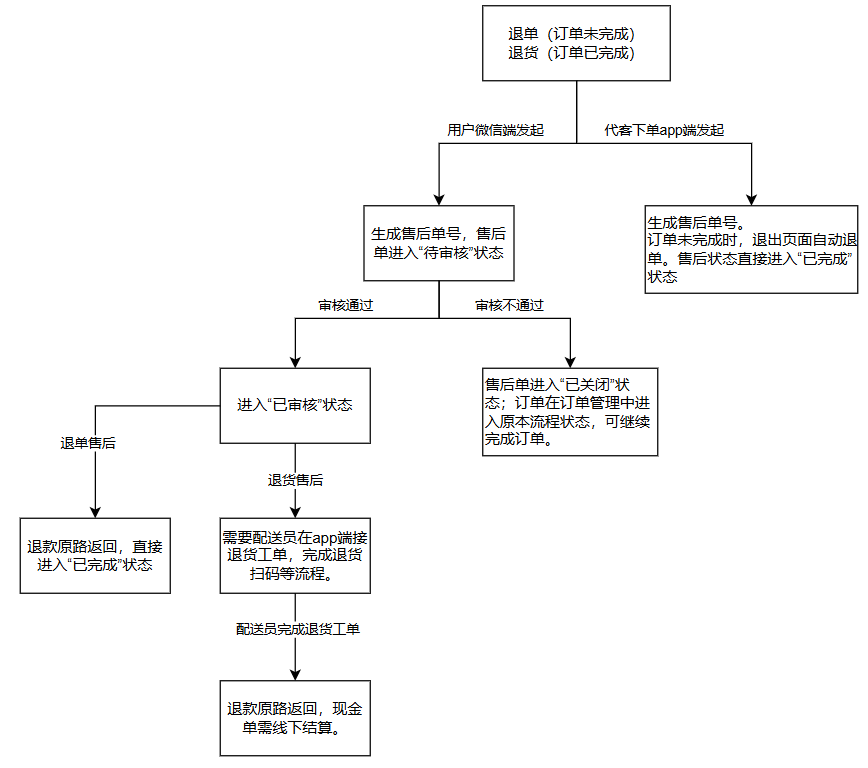
\includegraphics[width=1\linewidth]{dlh_tutorial_figs/chargeback}
	\caption{订单售后流程}
	\label{fig:chargeback}
\end{figure}


\subsection{回收}

从运气到家app端,首页-工单-回收,进入回收页面,若权限开放可新增回收项目。若只开放转派权限,则由客服接听电话时在网页端新增回收工单,派给配送员,从手机端接“回收”工单,配送员无法自主新增。

这一部分用法有限,并且难以监管,可根据公司实际运营要求使用。一般此类工单可走线下的现金和纸质单进行处理,线上单据对于无智能手机的用户来说非常不便。

\begin{itemize}
	
	\item 残液回收,公司不回收残液。气瓶残留的液化气到气站要抽残处理不做二次利用。
	
	\item 气瓶回收,可以根据公司要求的气瓶规格、年限定价,新增回收单。
	
	\item 商品置换,不知道置换什么。
	
\end{itemize}


\subsection{交易流水}

财务用的话可以写一下。


\section{工单}

\subsection{工单管理}

工单管理的分类可在“设置-工单配置-工单配置”中新增并启用。

\subsection{附加工单}



\section{设置}
作为网页的管理员,设置中的所有功能和页面都需要尽量熟悉,一些初始的配置和后续更新的功能,都可以在这个部分进行配置。该部分说明请结合实际网页功能查看。

\subsection{配送设置}

\begin{enumerate}
\item 订单分发规则

-预约派单时间,默认开启立即派单。关闭后可以设置预约单的派单时间。但如果手动派单的话应该是不受影响的,猜测是自动派单开启后,这里作为一个关联功能使用。

- 手动派单默认开启不能关闭,默认选中“上次处理人”,这个是手动派单时,派单界面自动填充上一个配送员,如无需修改即可一键派单。

- 自主抢单,这个有点像外卖和网约车的方式,利用手机GPS定位与订单位置,可设置位置区间自动派给订单区域内的配送员;并且可设置接单时间,超时自动再次分配。由于新郑公司给每位配送员定区域定责,因此未使用此功能。

- 自动派单,开启后可设置自动派单规则,一般将规则设置为“上次处理人”,配送员使用的好运气app必须为“接单中”状态。

- 自主配送单及工单分派方式设置,可以自主选择,在定户定责未完全落实的情况下需要保持手动派单;所有库房均已稳定配送用户后方可开启自动派单,减少派单任务量。

\item 配送附加工单

空的

\item 运费设置

可新增运费设置,根据不同楼层,选择递增或固定金额,无需运费的可将固定金额设为0。

\item 配送配置

- 随配送单关联安检,开启后在完成订单的“随单任务”里显示必做,完成后方可进入订单下一步操作。

- 随配送单合同签署,验证对应用户户号的用户是否已签署供气协议,即后续合同配置中上传的合同模板。若该户号的用户未签署过合同,则“随单任务”中会有这一项,若已签署合同,则不会出现该任务。

- 随配送单验证开户必填信息,字面意思。开户时一般会要求将必填信息填写后才完成开户。但开户必填信息是可以在系统上配置的,如果开户时有些信息非必填但是后续设置了必填,那这个功能开启时会验证并要求填写。

- 运气到家开启离线签单,这个功能网页中有详细解释,由于该功能开启后无法进行安检等必做任务无法完成,因此新郑公司未使用。

- 随配送单更新用户就近门店与订单门店,非常重要的功能,如果你需要统计用户数据,需要区分各库房任务,需要各库房营业员为老客户精准派单,这个功能可谓神来一笔,能解决大部分的问题,无脑开。

\end{enumerate}


\subsection{销售设置}
\begin{enumerate}
	\item 销售渠道设置
	
	保存了一些渠道名称和对应ID,可新增。平时用不到这个模块。
\end{enumerate}


\subsection{财务设置}
\begin{enumerate}
	\item 支付方式设置
	
	\begin{itemize}
		 
	\item 可按需将列举的支付方式更名、启用或停用。在对应的支付方式--编辑中,可配置相应的接口信息。

	\end{itemize}

	\item 支付渠道设置
	\begin{itemize}
		
		\item 微信商城支付配置,用户在微信上下单的各项付费业务的支付方式权限,可按不同部门配置权限。“微信商品下单启用货到付款”即不限制微信下单必须付款后再生成订单,权限按门店配置。
		
		\item 运气到家支付配置,送气工在app上代客下单时的各项付费业务的支付权限,可按不同部门配置权限。
		
		\item 平台支付配置,网页端客服或营业员下单时的支付配置。
		
	\end{itemize}



\end{enumerate}


\subsection{微信配置}
\begin{enumerate}
	\item 一键订气配置
	
	配置“微信订气”首页的界面组件。可在中间界面图片中点击对应位置的组件,并在右侧显示的组件详情中自行配置。其中,左侧的组件库也可拖拽至中间界面图片想要的位置中,自行配置页面布局。
	
	\item 个人中心配置
	
	配置“微信订气”中“个人中心”的功能模块。可自行配置所需显示给用户的功能,以及显示位置。但是“发票”功能是2024.12月的新功能,新郑公司未使用,因此未对使用方式进行了解。
	
	\item 公众号配置
	
	这个是公司申请服务号后由多立恒配置新增。
	
	\item 微信业务配置
	
	配置微信订单的待支付时限;配置微信端配送中是否显示配送员详细信息,姓名、电话号码等。
\end{enumerate}


\subsection{工单配置}
\begin{enumerate}
	\item 工单配置
	在好运气app首页的“工单”中列出的工单选项。
	报修、
	投诉、
	咨询。
	可按需新增,新郑公司在该模块中新增了“沉睡气瓶排查单”工单,用于上传沉睡气瓶告知书,保存相应的用户信息与告知书下发原因。
	
	\item 附加工单配置
	
	附加工单配置可自行新增,附加工单启用是也是在在好运气app首页的“工单”中显示。
	
	
\end{enumerate}



\subsection{安检配置}
\begin{enumerate}
	\item 安检模板配置
	
	\begin{itemize}
		

	\item 定期安检和随单安检有区分,随单安检是订单完成中的随单任务,定期安检是好运气app首页“安检”一栏入口的安检。
	
	\item 安检模板配置--编辑:可设置安检单名称,选择适用用户类型,适用用户门店,以及安检周期。如果不同门店或不同类型用户的安检内容不一样,可以复制新增多个安检模板,并在对应模板内修改。安检周期设置后,如果用户上次安检时间超过了设置的时间,用户在微信订气的“个人中心”中会显示“安检已超期”字样,网页上用户安检的信息中也会有同样提示。可根据公司的管理制度决定是否需要配送员上门进行定期安检。
	
    \item 安检模板配置--安检项配置:可根据地区的相关法律法规新增安检项,可为安检项的每个条目设置隐患等级,如需整改,可自定义整改意见。隐患等级以及是否需要整改可在“隐患配置”中配置。
	
	\end{itemize}
	
	\item 隐患配置
	\begin{itemize}
		\item 
	
	可新增或设置隐患名称,是否需整改,以及状态是否启用。用于安检模板中的安检项隐患选项。
	\end{itemize}
	\item 其他配置
	
	\begin{itemize} 
	
	\item 位置异常标记,可设置安检位置超出用户地址的距离,设置并保存后,安检单管理中“位置偏差”一列会显示实际超出的距离。未超出的不显示。
	
	\item 定期安检审核,随单安检审核。这两个功能开启后在“安检单管理”中,每条安检信息后会有“审核”功能,需要在网页中手动审核,方可在流程中完成整个安检。开启审核后,据说未审核的安检单仍可以修改安检中的勾选选项。至于修改方法因未使用过,所以暂时不了解。
	
	\item 整改审核,有隐患的安检单会在配送员的好运气app上保留一个整改任务,若通过这个整改入口重新整改勾选安检项,提交后仍需“审核”。
	
	\item 随单安检更新用户上次安检时间,“用户管理”页面中的用户信息有一个“上次安检时间”,如果这个配置开启,那么手动审核后才会在这一列更新上次安检时间,否则不会更新。
	
	\item 安检后立即更新用户安检时间,这个功能开启后无需依赖手动审核,安检时间直接根据安检的提交时间上传更新在用户管理中的“上次安检时间”位置。
	\end{itemize}

\end{enumerate}


\subsection{用户配置}
\begin{enumerate}
	\item 开户设置
	
	设置开户信息模板,可编辑。
	
	\item 用户类型
	
	用户类型可新增,可编辑。该模块会影响所有用户类型相关查询,商品或安检的适用用户类型等。
	
	\item 开户配置
	
	开户配置:开户后自动创建工单,有需要的可以用。实名开户配置,这个配置主要是实名认证需求,比如工业用户,按公司管理要求可开启企业或个人的信息认证。开启后,用户选择工业类型,则个人或企业信息会成为必填项,用户需填写后方可成功开户。
	
	开户须知:开户须知可自行编辑填写。
	
	\item 用户标签
	
	可自行配置,一般无特殊需求可以不设置。
	
	\item 合同模板管理
	
	可新增合同。\textcolor{red}{(不太会用,我上传pdf的时候会提示“文本域或关键字为空”)}	
	
\end{enumerate}

\subsection{溯源配置}
\begin{enumerate}
	
	\item 一户一码配置
	
	这个功能配置的是每个用户户号对应的唯一二维码扫码时展示的页面。
	
	\begin{itemize}
		\item 组件库,可将相应的组件名称拖拽至UI界面的相应位置,自定义搭配。
		\item 轮播图片,界面最上端图片最多可轮播6张图片,建议长宽比3:1。
		\item 用户信息,可自定义该界面展示的用户信息,包含用户基础信息以及部分用气信息。
		\item 在用气瓶信息,展示现场配送节点在对应用户处的气瓶,包含气瓶编号与芯片编码。
		\item 用气统计,可按时间区间展示最多近1年的订气瓶数。
		\item 配送信息,可选择展示最近x次配送,可选显示字段“配送时间”,“配送车辆”,“配送员”。
		\item 安检信息,可选择展示最近x次安检。该模块在实际界面中可点击“详情”查看详细安检情况。
		\item 订气渠道入口,可勾选两种渠道,“电话订气”、“微信订气”。
	\end{itemize}
	
	\item 一瓶一码配置
	
	这个功能配置的是瓶身安装的已建档的芯片二维码扫码时展示的页面。
	
	\begin{itemize}
		\item 组件库,可将相应的组件名称拖拽至UI界面的相应位置,自定义搭配。
		\item 页面标题,标题可自定义。
		\item 轮播图片,轮播图片,界面最上端图片最多可轮播6张图片,建议长宽比3:1。
		\item 使用预警,用户气瓶超时未流转不合格预警设置。可自定义搭配用户类型、气瓶类型、超时天数设置预警信息,可新增多个预警条件。相应用户类型、气瓶类型超期的气瓶,扫描瓶身二维码时会显示使用预警信息以及显眼的“疑不明气源”红码标识。
		\item 气瓶信息,可勾选列举的所有气瓶信息,该信息详情与网页内气瓶建档导入的信息关联,与气瓶厂家出厂信息不直接相关。
		\item 流转信息,所有流转信息可勾选展示,可公司实际管理要求勾选具体的展示类别和每个类别内展示的具体项目。这个信息的详细内容因为是一个气瓶完整的追溯项目,所以建议完整查看一遍。
	\end{itemize}
	
	
	\item 一车一码配置
	
	这个功能配置的是网页中 配送--车辆管理 中,新增车辆生成的唯一二维码扫码时的展示页面。
	\begin{itemize}
		\item 组件库,可将相应的组件名称拖拽至UI界面的相应位置,自定义搭配。
		\item 车辆信息,此信息与 配送--车辆管理 中的录入信息关联,可自定义配置可扫码获得的数据项。
		\item 员工信息,此信息包含“司机”与“押运员”,车辆管理-新增车辆 时,需从系统账号管理已有的人员中选择人员作为司机和押运员,人员对应信息与账号管理中写入的信息关联。可自定义配置扫码获得的数据项。
		\item 库存详情,可展示该车辆中存放的重瓶、空瓶,及其对应的规格、数量、气瓶号、芯片编码。该信息与气瓶流转信息关联,若流转扫码节点最终位置在车辆对应的配送员或司机处时,气瓶信息将会更新至车辆的库存信息中。
		\item 配送信息,与气瓶流转信息关联,车辆对应的配送员送出扫码时更新此项目数据。
		\item 预警信息,目前不清楚使用场景与关联更新模块。
	\end{itemize}
	
	
\end{enumerate}

\end{document}














